% Latex template: mahmoud.s.fahmy@students.kasralainy.edu.eg
% For more details: https://www.sharelatex.com/learn/Beamer

\documentclass{beamer}					  % Document class

\usepackage[portuguese]{babel}			  % Set language
\usepackage[utf8x]{inputenc}			  % Set encoding

\mode<presentation> {					  % Set options
  \usetheme{default}					    % Set theme
  \usecolortheme{default} 				% Set colors
  \usefonttheme{default}  				% Set font theme
  \setbeamertemplate{caption}[numbered]	% Set caption to be numbered
}

\setbeamertemplate{navigation symbols}{}
\setbeamertemplate{footline}[frame number]
\setbeamercovered{transparent}

% Uncomment this to have the outline at the beginning of each section highlighted.
%\AtBeginSection[]
%{
%  \begin{frame}{Outline}
%    \tableofcontents[currentsection]
%  \end{frame}
%}

\usepackage{graphicx}					% For including figures
\usepackage{booktabs}					% For table rules
\usepackage{hyperref}					% For cross-referencing
\usepackage{caption}                    % Allows more control over captions in figs and tables

\title{Revisão de Atividades da FAC}	% Presentation title
%\author{Author One}					% Presentation author
\institute{LNLS.DAC.FAC}				% Author affiliation
\date{2024-12-12 -- 2024-01-26}			% Today's date	


\begin{document}



\begin{frame}
  \titlepage
  \href{https://github.com/lnls-fac/doc-review-dac-fac}{\beamergotobutton{Link para o repo github desta apresentação: https://github.com/lnls-fac/doc-review-dac-fac}}
  \href{https://www.overleaf.com/read/sbdjxtzfchrm}{\beamergotobutton{Link para o projeto overleaf destas notas}}
\end{frame}

\begin{frame}{Outline}
  \tableofcontents
\end{frame}


\section{PU em standby no Topup}

\begin{frame}{PU em standby no Topup}
    \scriptsize{\begin{itemize}
            \item 50\% tensão, 100\% faltando 20s para injeção
    		\item Em 2024-01-24 (quarta) habilitamos o standby dos PU
            \item Eficiência de injeção no anel piorou, pequenos ajustes de tensão no NLK
            \item Piora sensível na repetibilidade da eficiência (mas sem afetar a corrente do Feixe)
    \end{itemize}}
    \begin{figure}[H]
        	\centering
            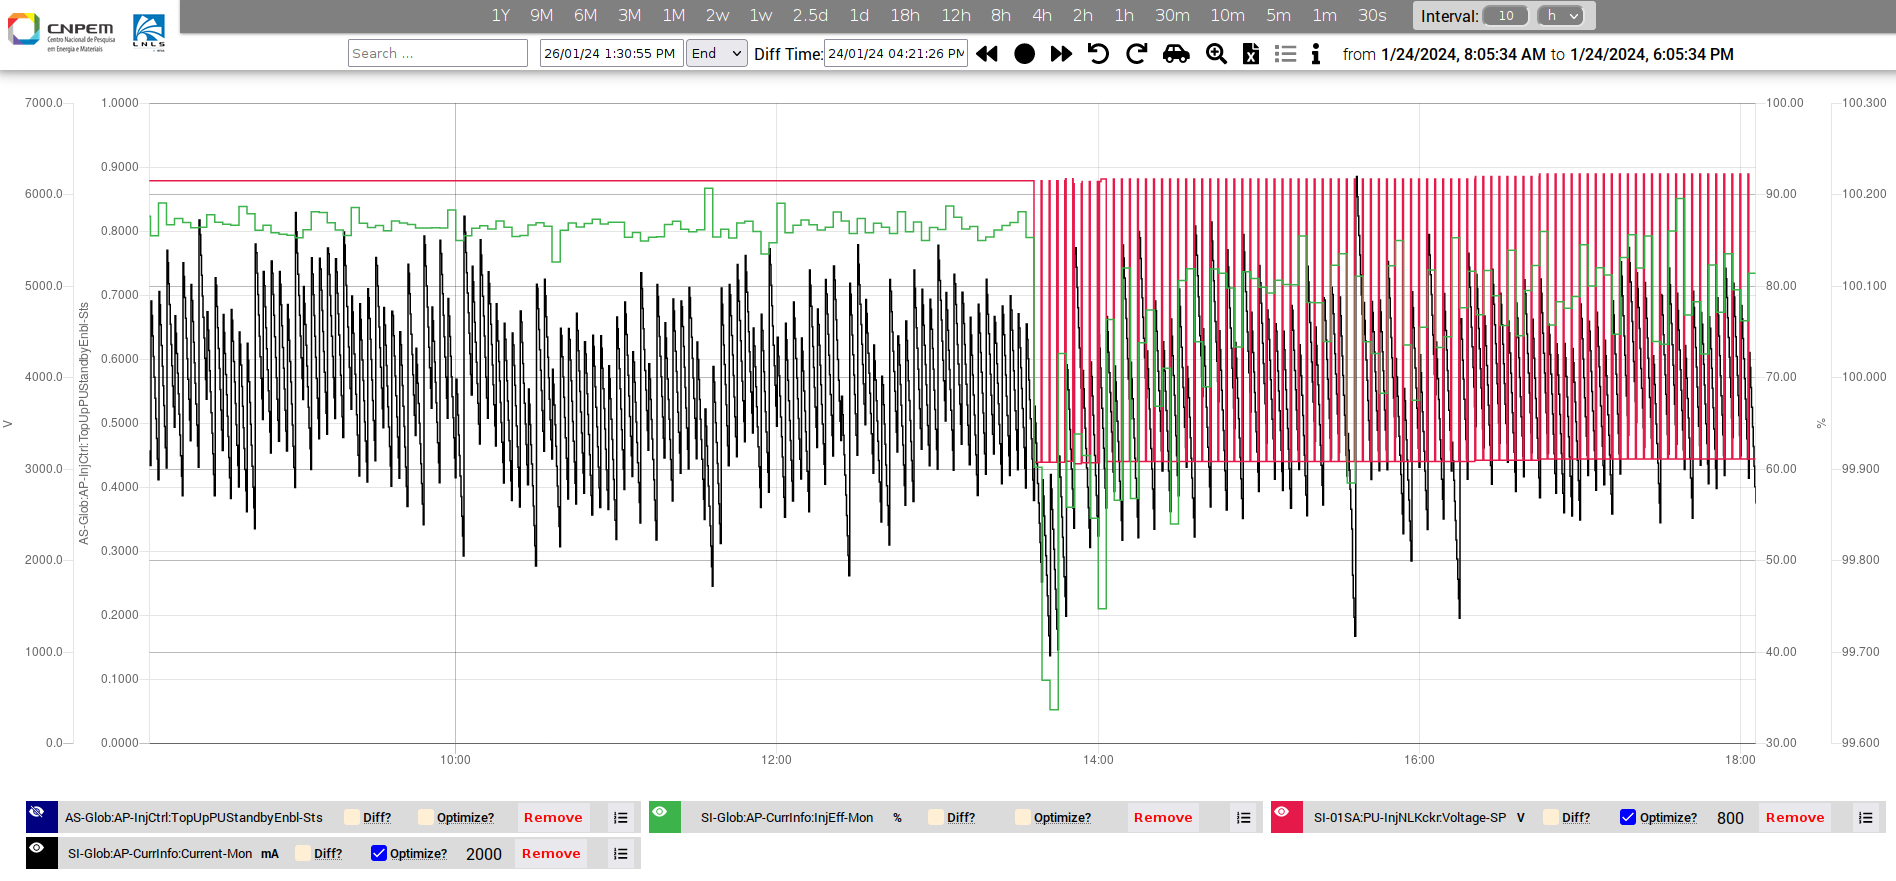
\includegraphics[width=0.8\textwidth]{2024-01-26/figures/pu-standby.png}
            \label{fig:pu-standby}
    \end{figure} 
\end{frame}


\section{NLK}

\begin{frame}{NLK - kick horizontal}
    \scriptsize{\begin{itemize}
    		\item Feixe localizado
            \item Varredura do pulso NLK com relação ao feixe
    \end{itemize}}
    \begin{figure}[H]
        	\centering
            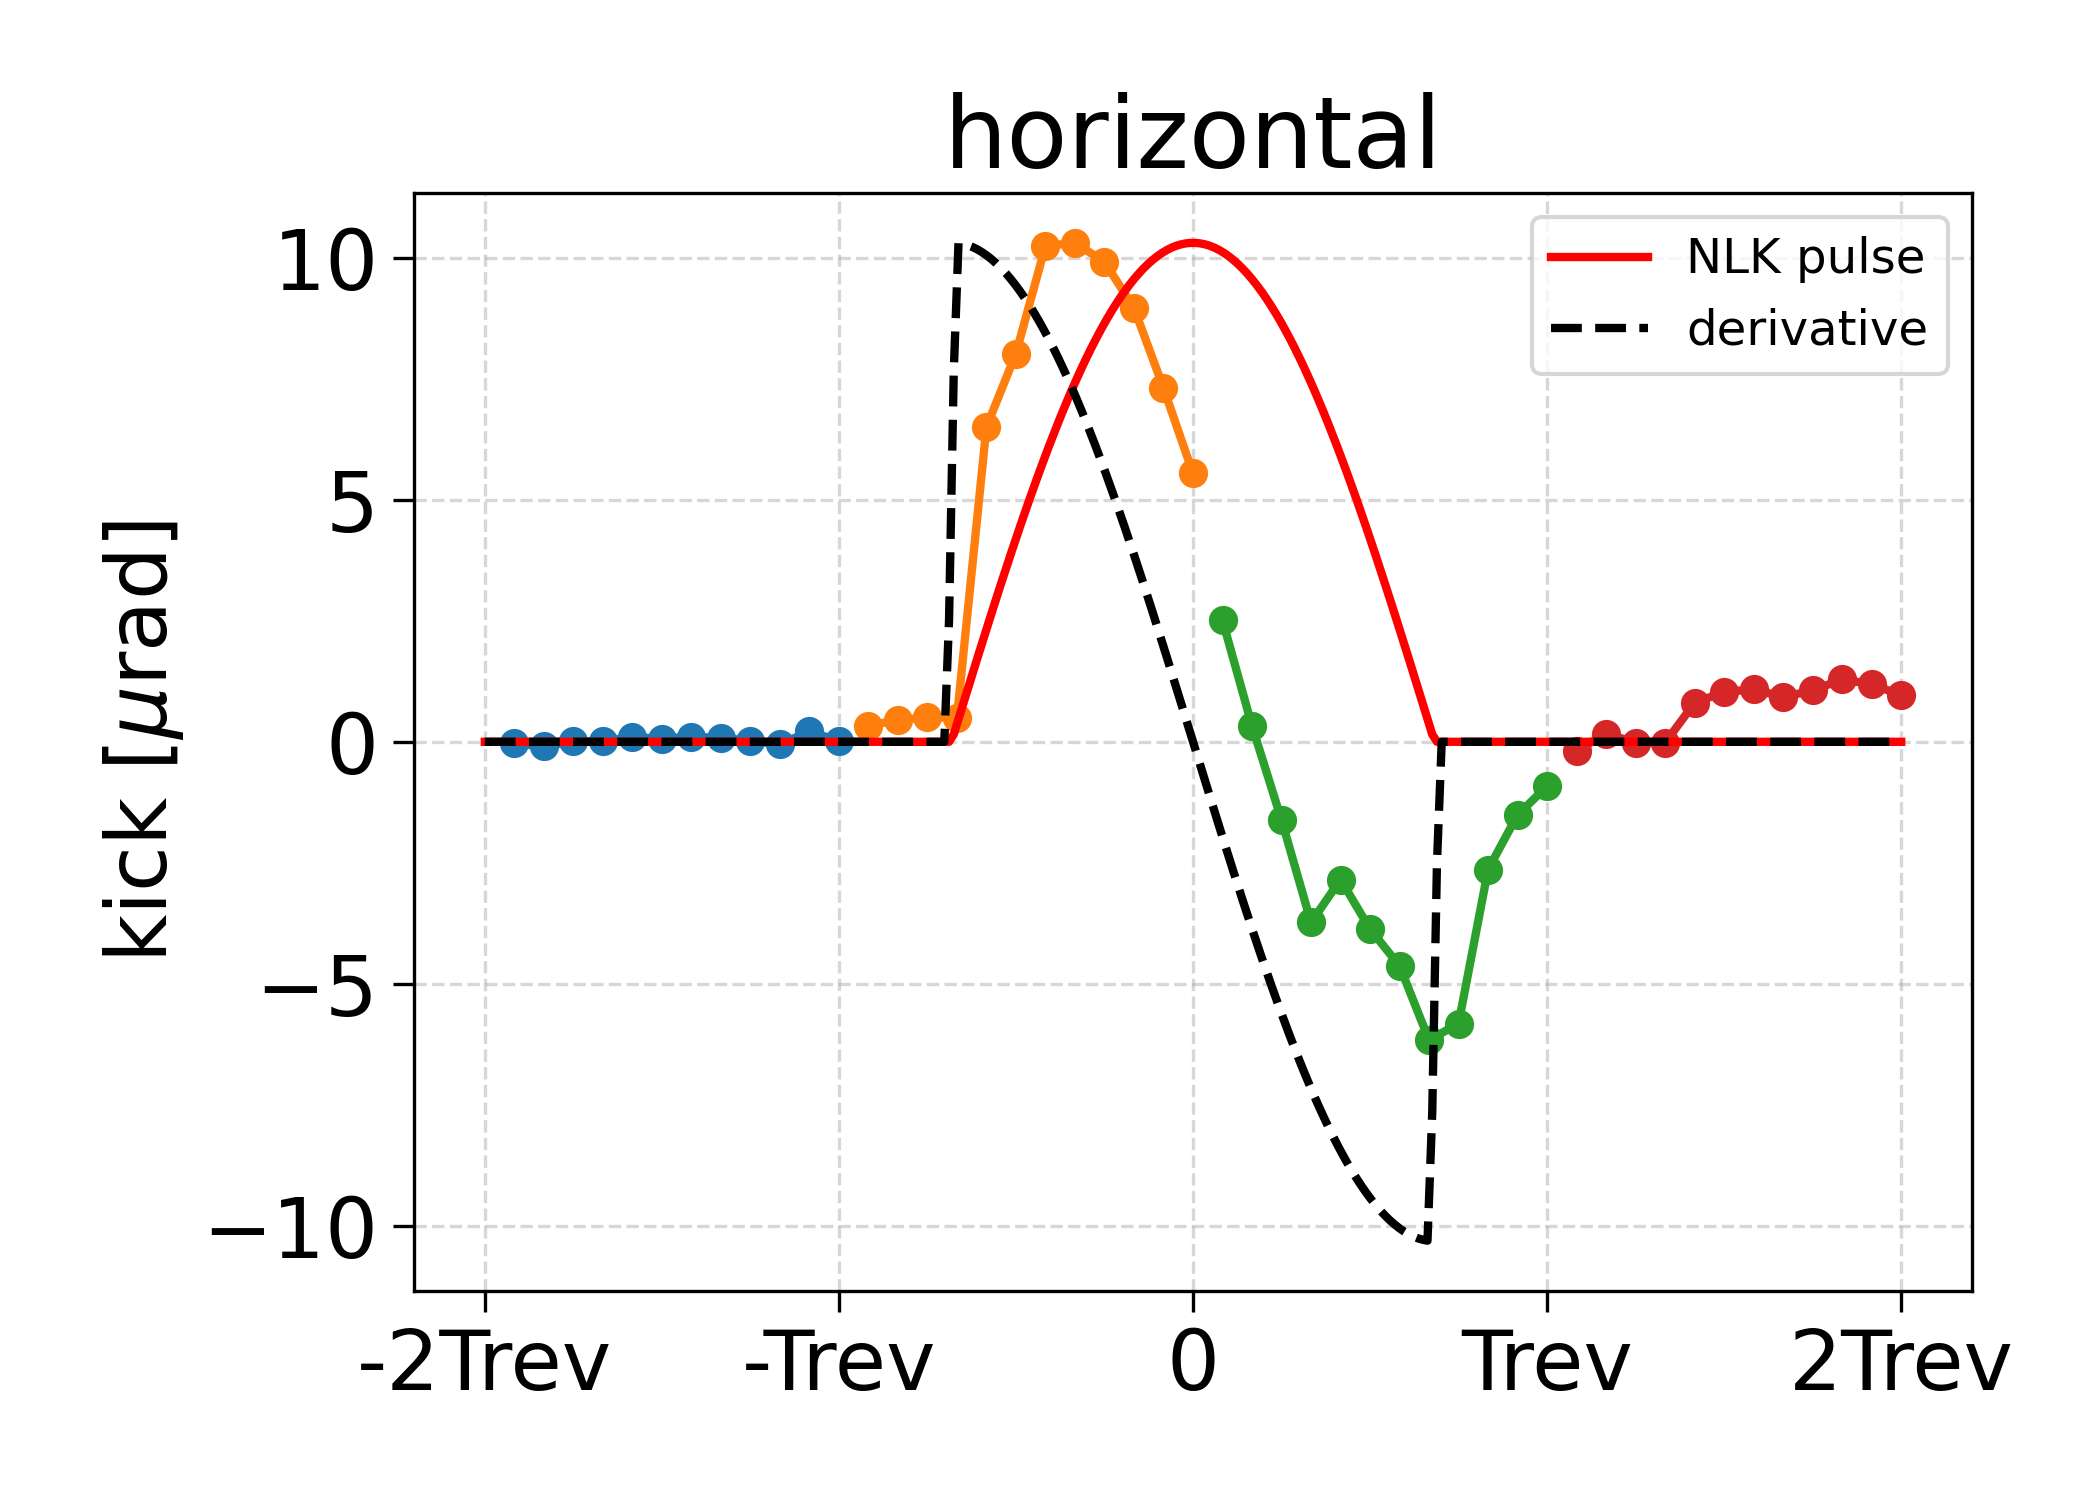
\includegraphics[width=0.8\textwidth]{2024-01-26/figures/nlk_horizontal_kick_profile.png}
            \label{fig:nlk-h-kick-profile}
    \end{figure} 
\end{frame}

\begin{frame}{NLK - kick vertical}
    \scriptsize{\begin{itemize}
    		\item Feixe localizado
            \item Varredura do pulso NLK com relação ao feixe
    \end{itemize}}
    \begin{figure}[H]
        	\centering
            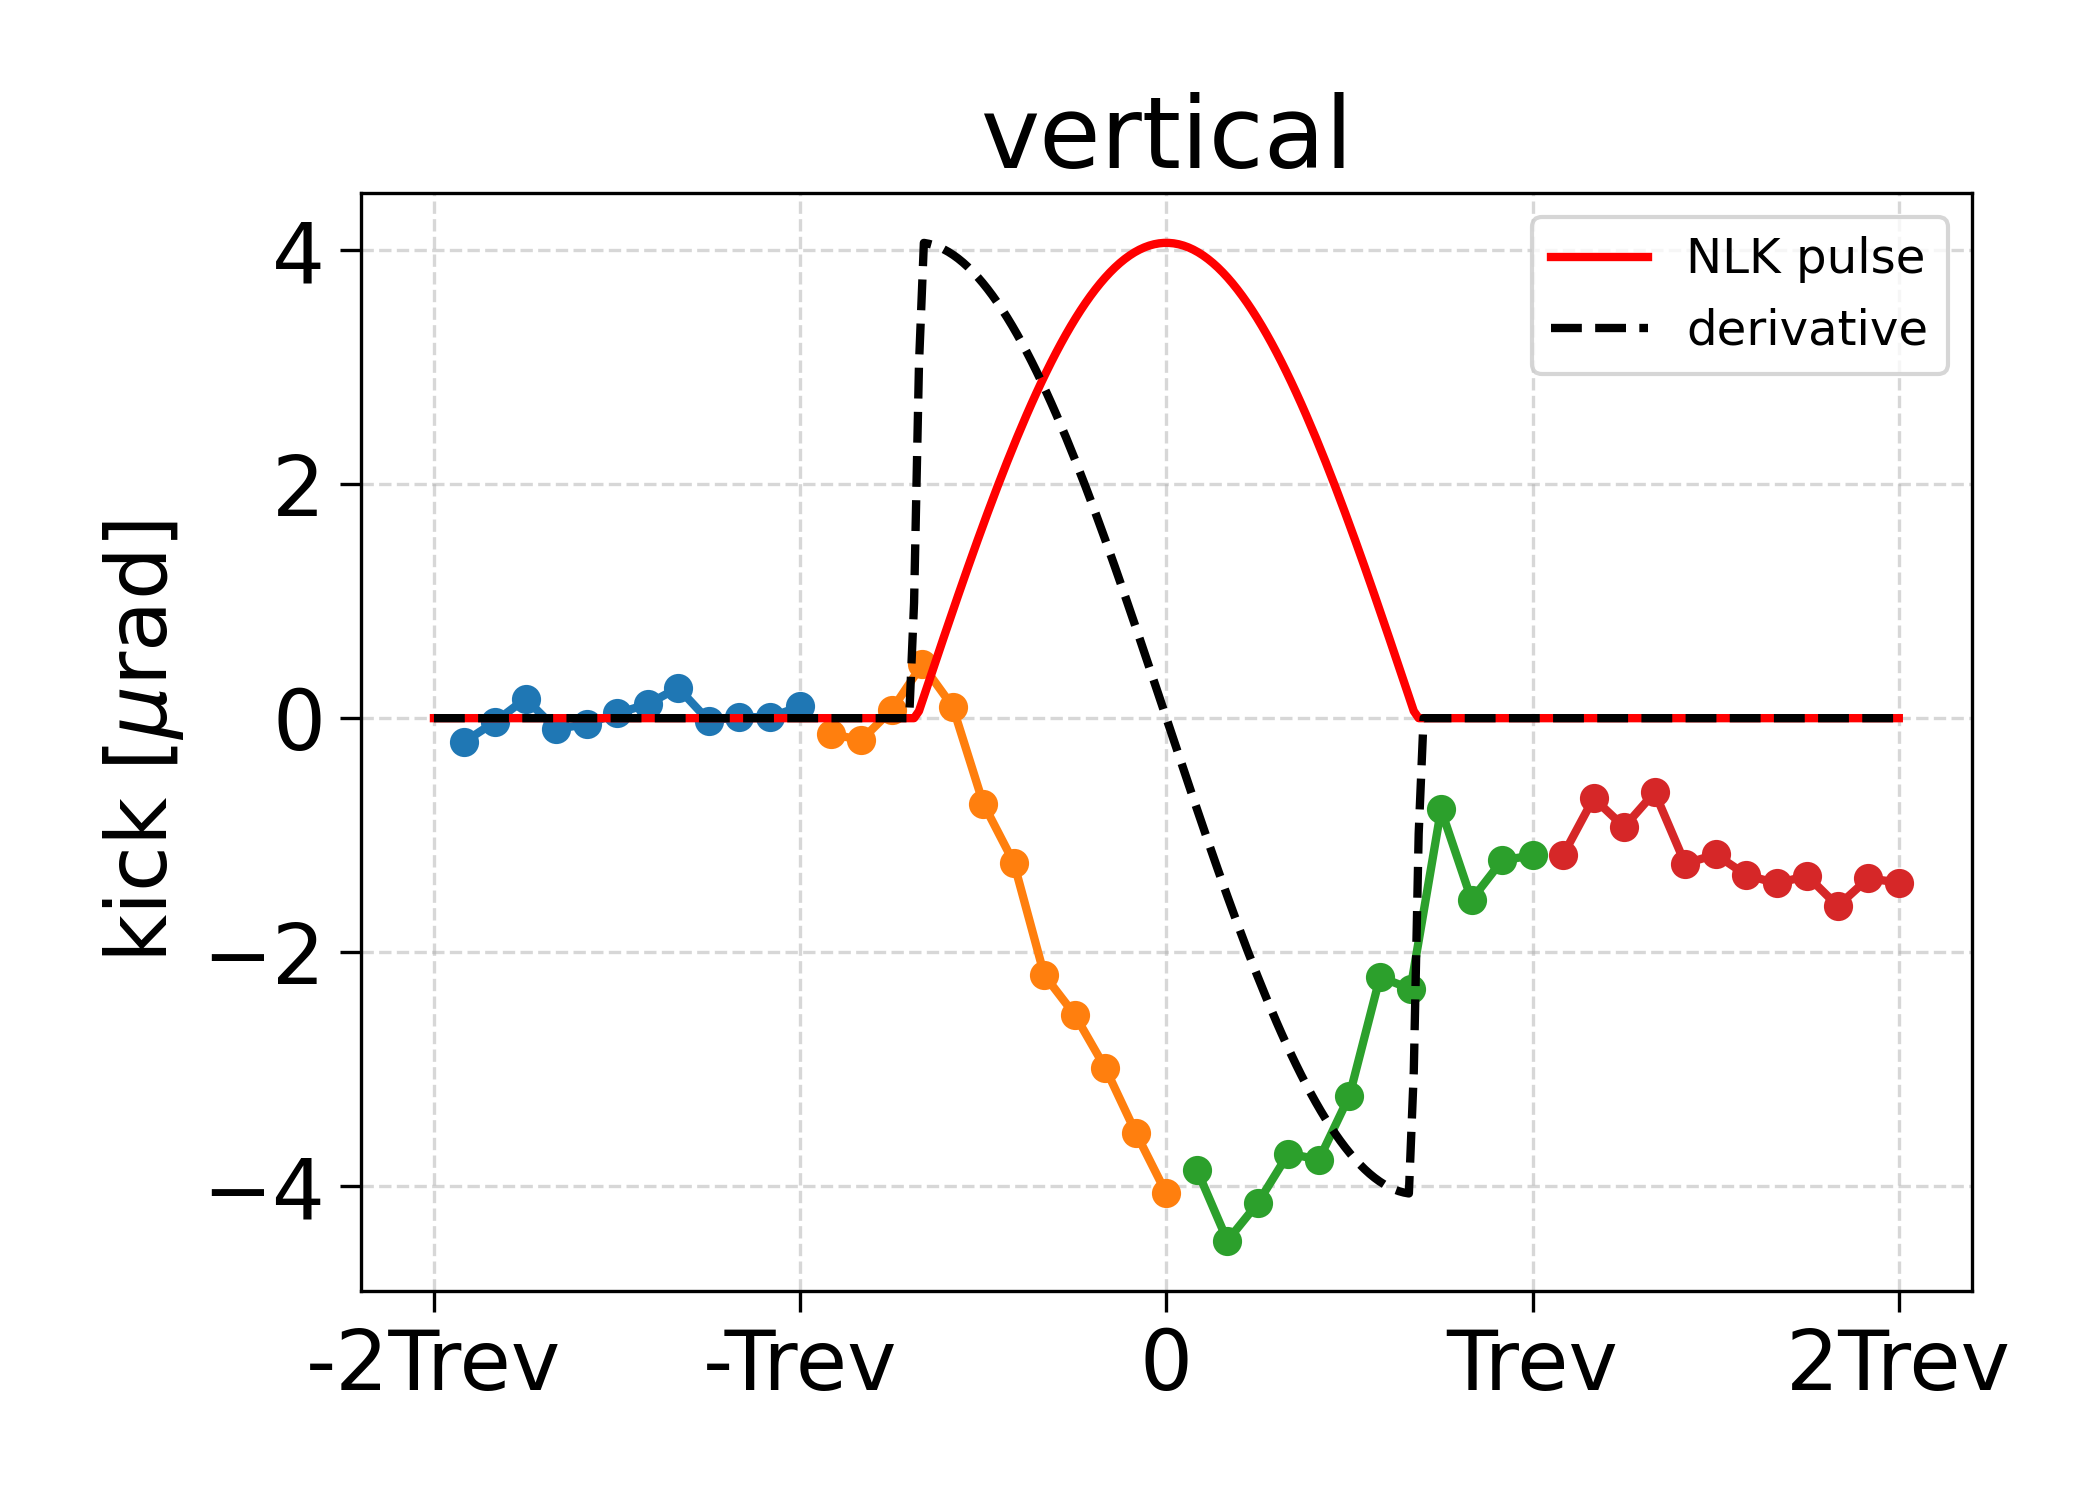
\includegraphics[width=0.8\textwidth]{2024-01-26/figures/nlk_vertical_kick_profile.png}
            \label{fig:nlk-v-kick-profile}
    \end{figure} 
\end{frame}

\begin{frame}{Comparativo da perturbação no centroide (BPM-01M2)}
    \begin{figure}[H]
        	\centering
            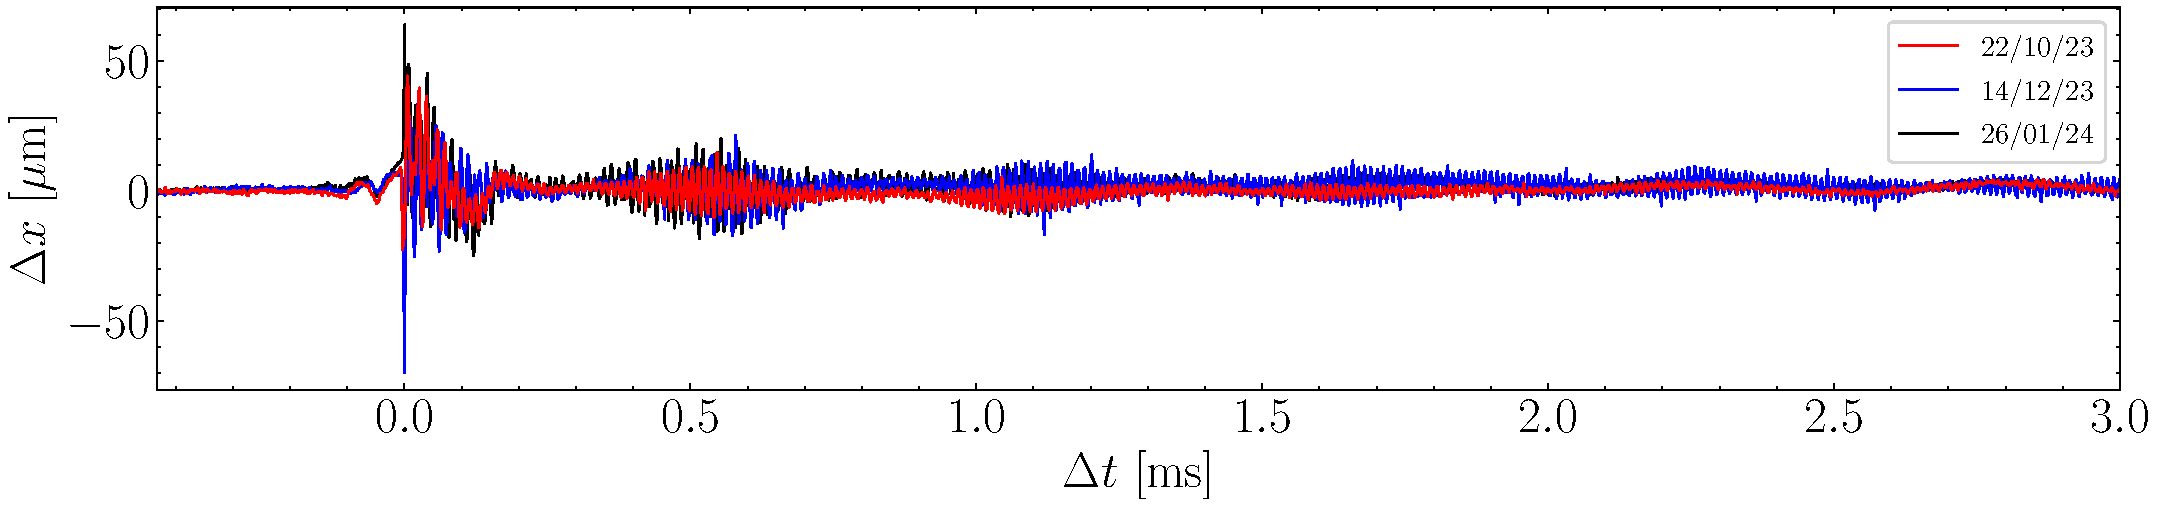
\includegraphics[width=1.0\textwidth]{2024-01-26/figures/injection_perturbation_compare_x_2024.pdf}
            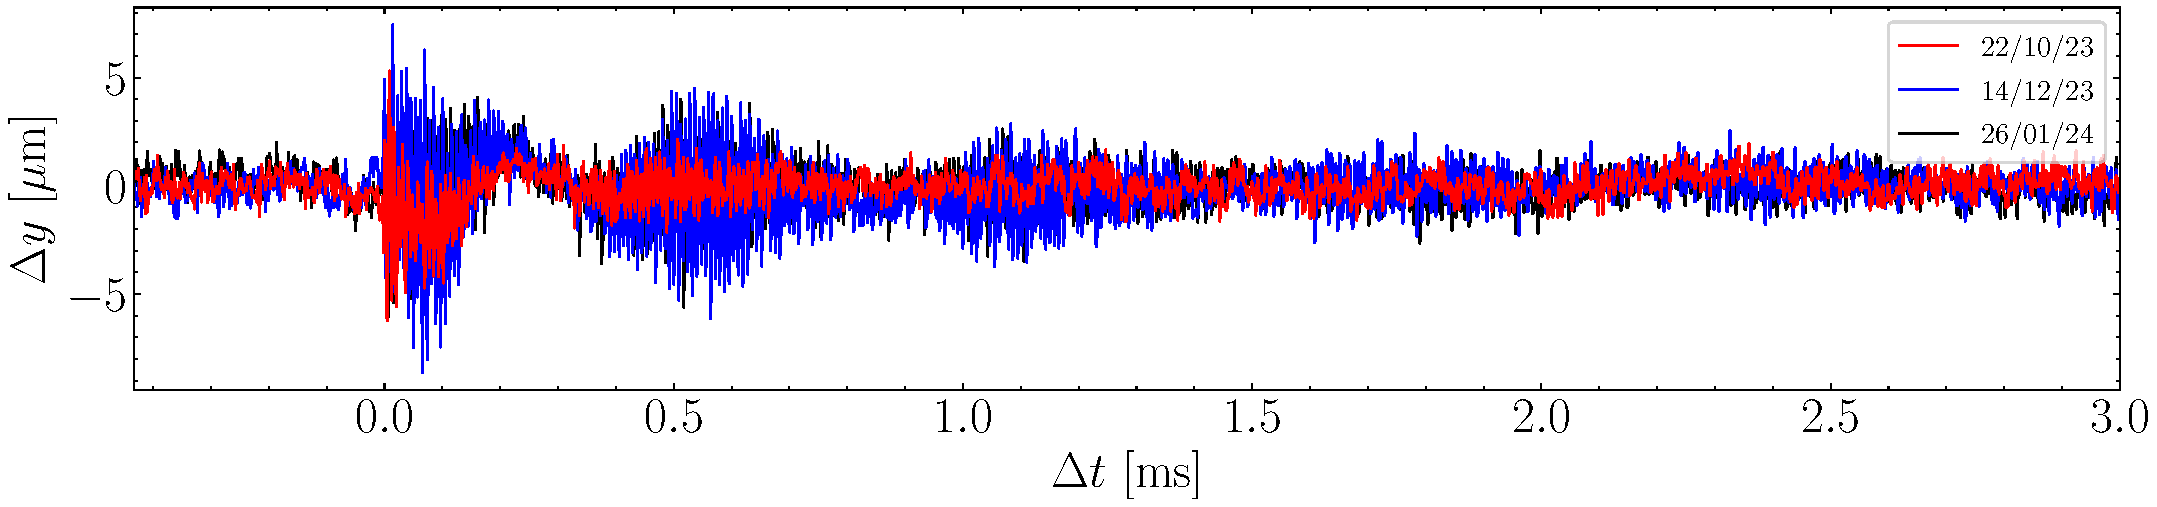
\includegraphics[width=1.0\textwidth]{2024-01-26/figures/injection_perturbation_compare_y_2024.pdf}
    \end{figure} 
\end{frame}

\section{Estudos com o DELTA52}

\begin{frame}{DELTA52 - Caracterização e Correção}
    \begin{figure}[H]
    		\centering
            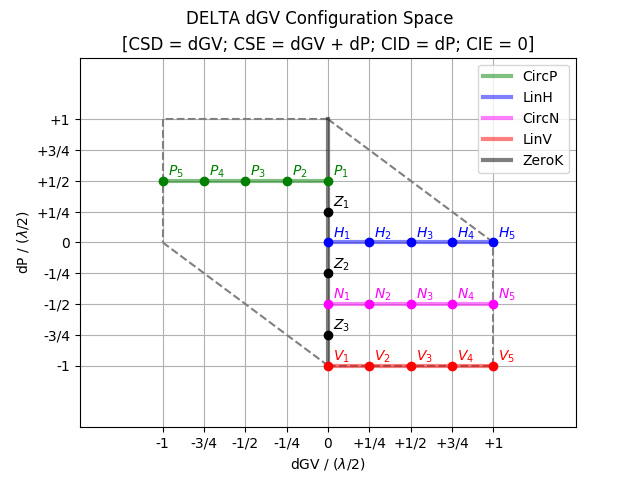
\includegraphics[width=.8\textwidth]{2024-01-26/figures/id-delta-dgv-config-space.png}
            \caption{Espaço de configuração do DELTA}
            \label{fig:delta-config-space}
    \end{figure}
\end{frame}

\begin{frame}{DELTA52 - Caracterização e Correção}
    \begin{itemize}
    		\item Movimentação do DELTA provoca a) distorções de órbita, b) mudança de acomplamento, c) distorção das funções beta, d) mudança da abertura dinâmica, tempo de vida, tc.
            \item Todos estes efeitos afetam a matriz resposta de órbita.
            \item correção local com pares de CHs, CVs, QSs, trims QFB, QDB1 e QDB2.
    \end{itemize}
    \begin{figure}[H]
        	\centering
            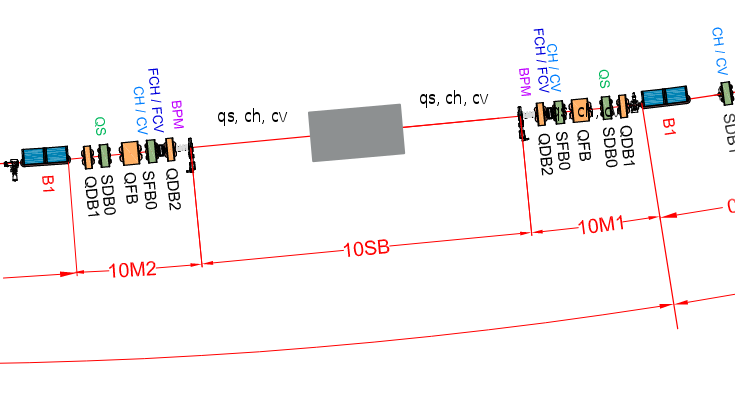
\includegraphics[width=0.6\textwidth]{2024-01-26/figures/si-10sb-2.png}
            \caption{\small{8 botões: 2 CHs, 2 CVs, 1 QS, QFB1, QFB, QDB2}}
            \label{fig:bba}
    \end{figure}
\end{frame}


\begin{frame}{DELTA52 - Caracterização e Correção}
    \begin{itemize}
    		\item Quadrupolos fitados (iteração 0)
    \end{itemize}
    \begin{figure}[H]
        	\centering
            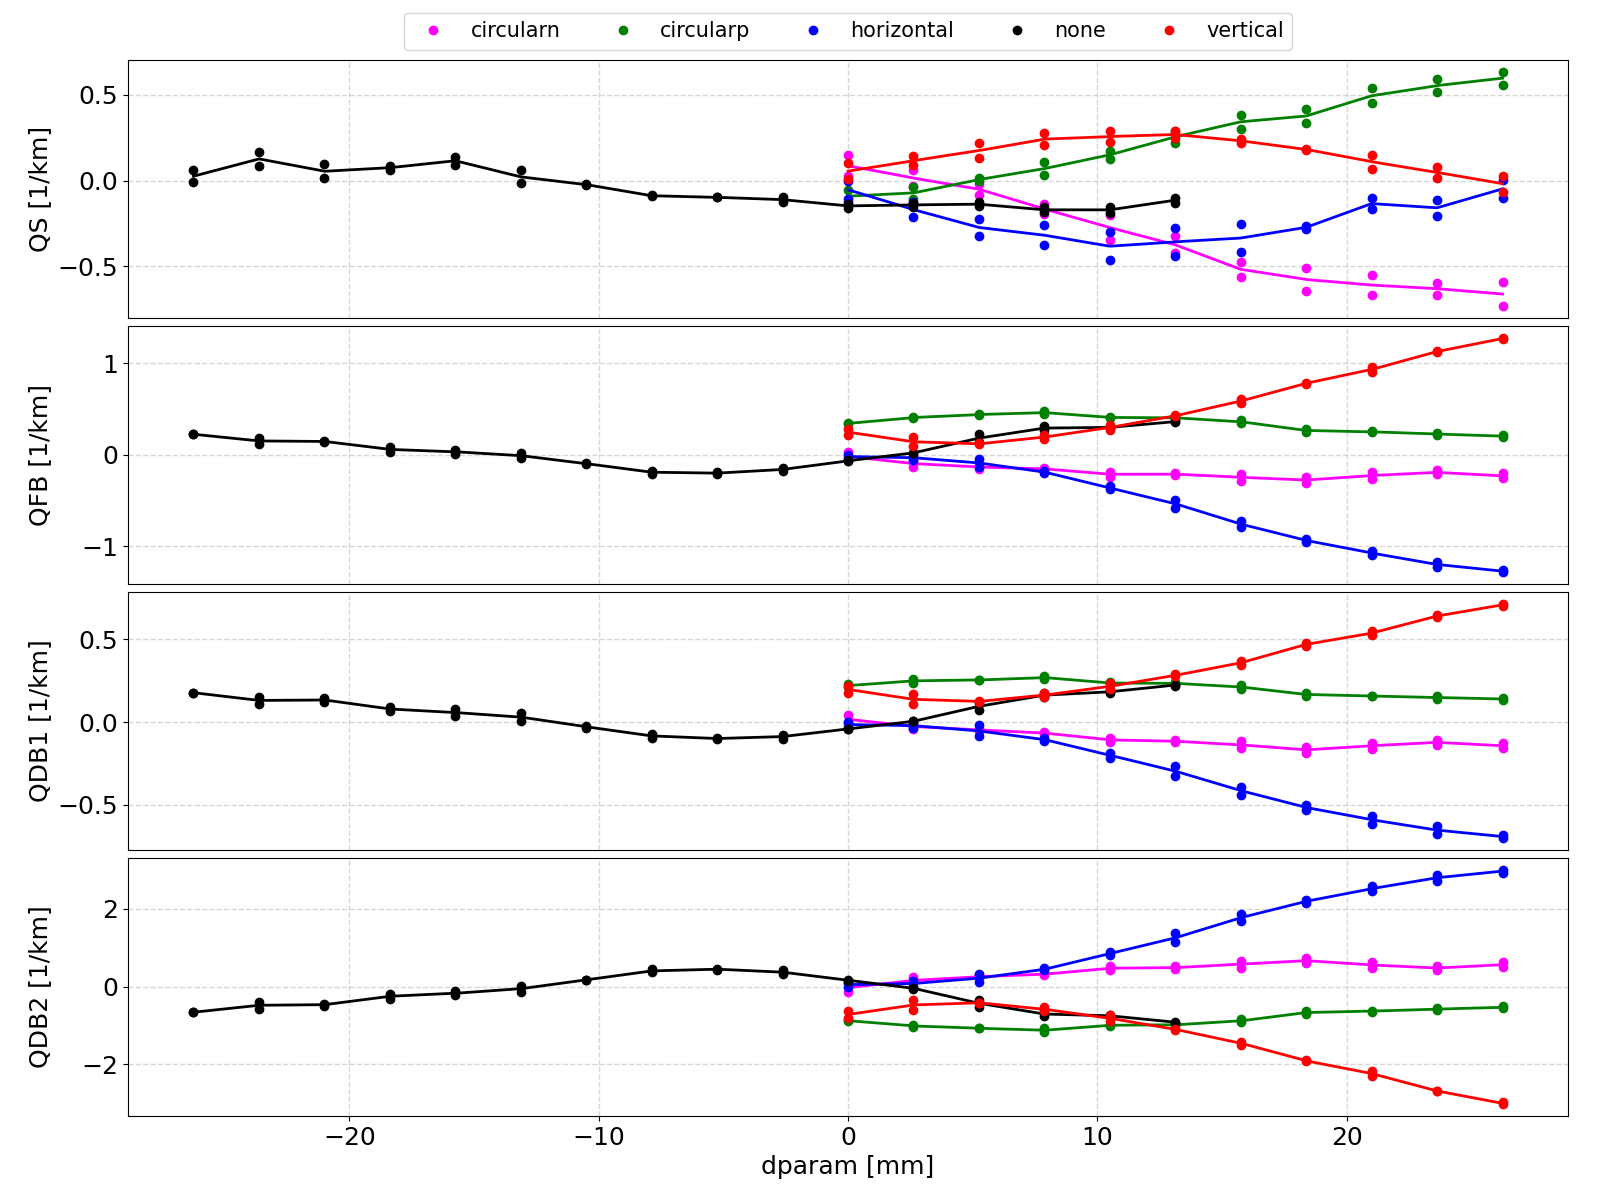
\includegraphics[width=0.8\textwidth]{2024-01-26/figures/knobs-before.png}
            % \caption{\small{No correction}}
            \label{fig:bba}
    \end{figure} 
\end{frame}


\begin{frame}{DELTA52 - Caracterização e Correção}
    \begin{itemize}
    		\item Efeitos da correção na emitância vertical (calculado modelo calibrado).
    \end{itemize}
    \begin{figure}[H]
        	\centering
            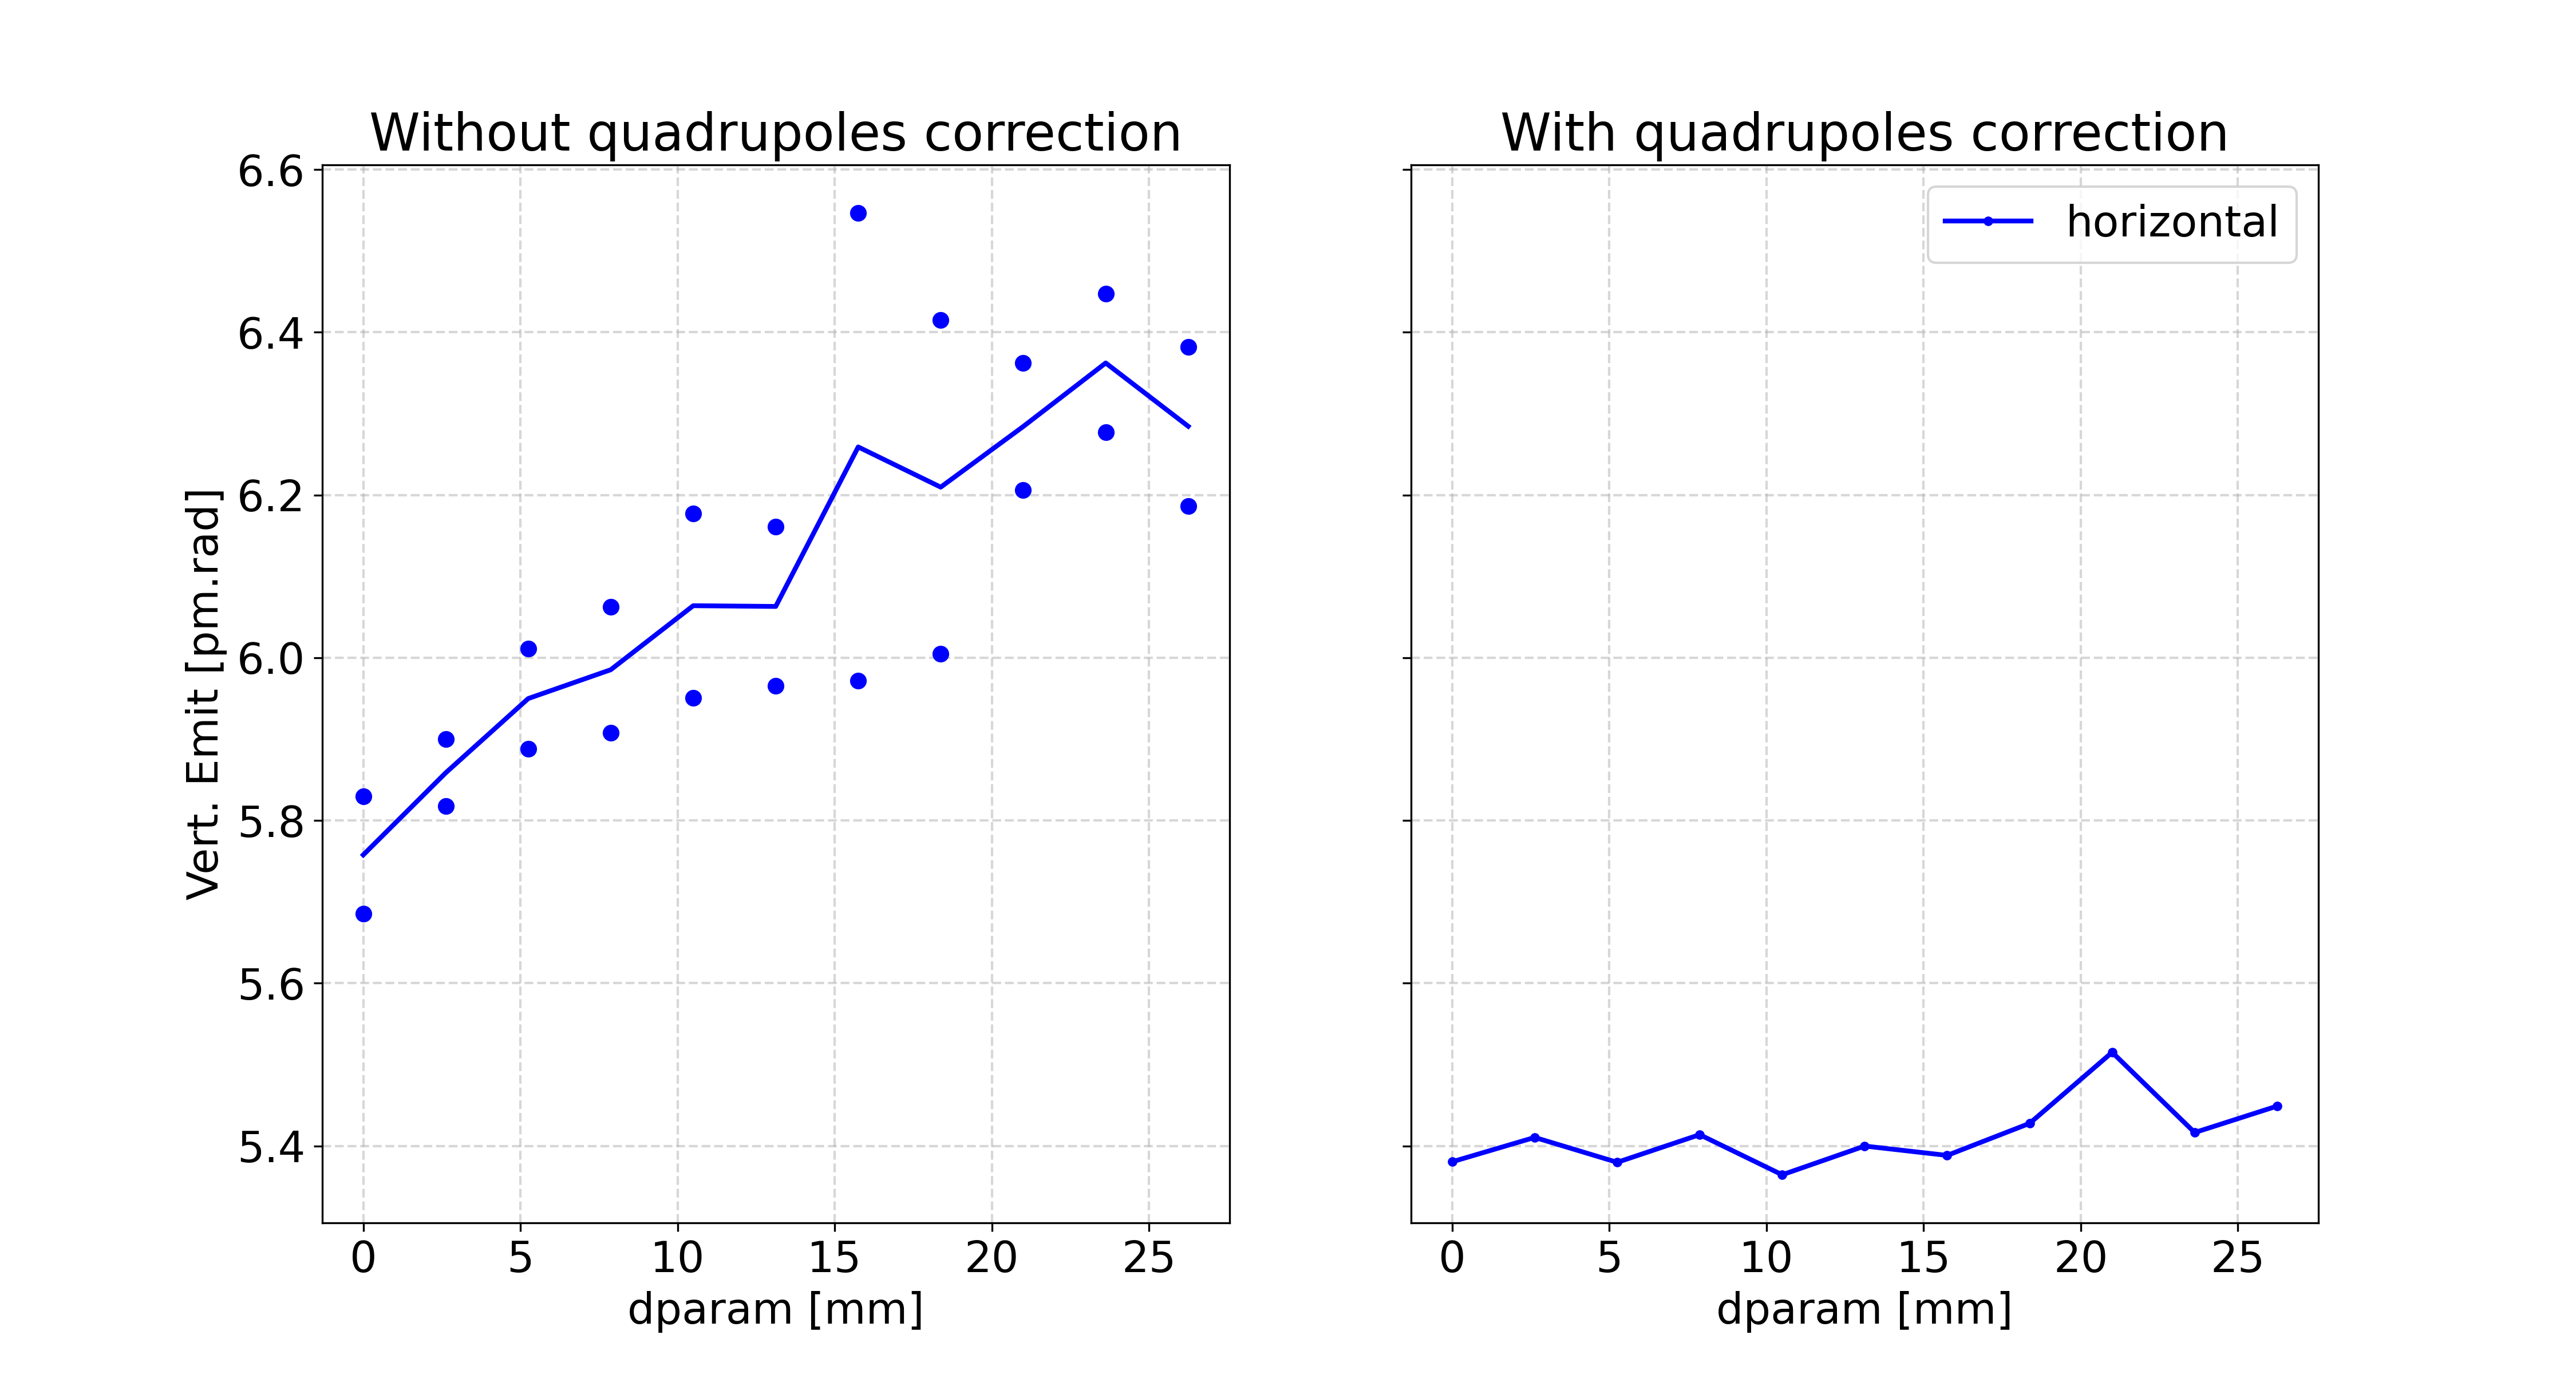
\includegraphics[height=4.5cm, width=9cm]{2024-01-26/figures/quad_ffwd_emit_effect.png}\\ 
    \end{figure} 
\end{frame}


\begin{frame}{DELTA52 - Caracterização e Correção}
    \begin{itemize}
    		\item Efeitos da correção nos desvios de sintonia (medidos).
    \end{itemize}
    \begin{figure}[H]
        	\centering
            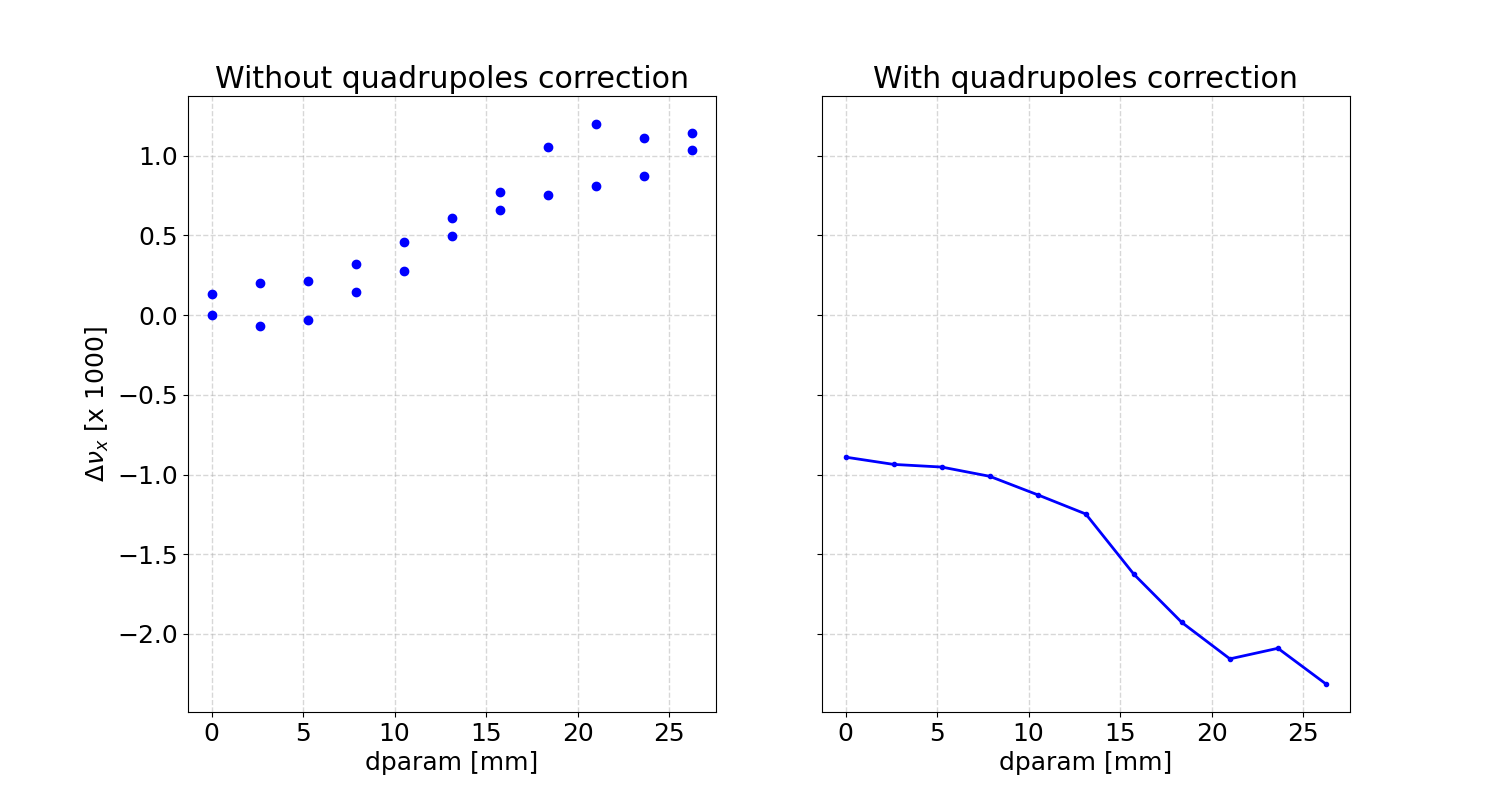
\includegraphics[height=3.5cm, width=9cm]{2024-01-26/figures/loco_tunex_corr.png}\\ 
            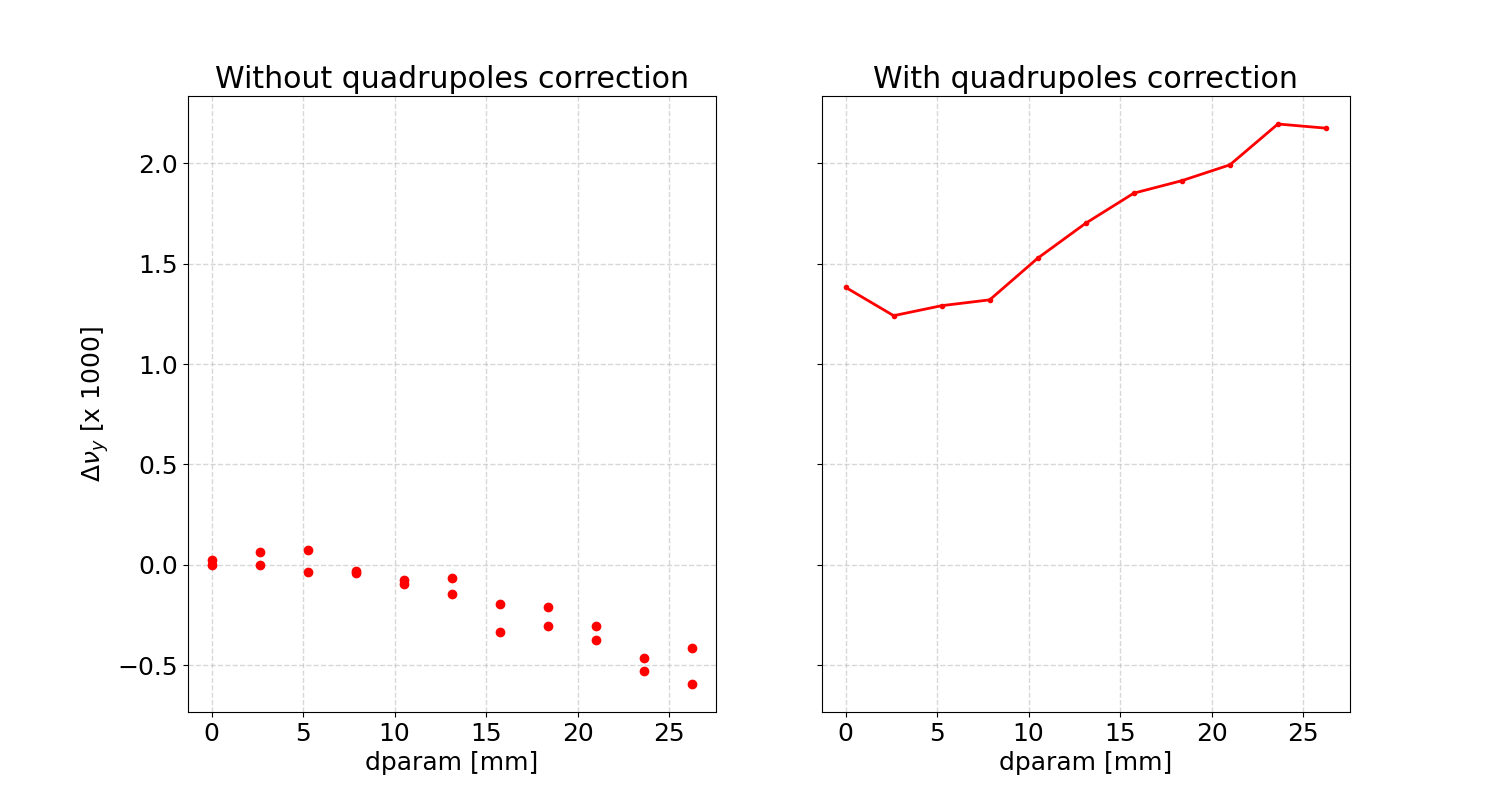
\includegraphics[height=3.5cm, width=9cm]{2024-01-26/figures/loco_tuney_corr.png}\\ 
    \end{figure} 
\end{frame}


\begin{frame}{DELTA52 - Caracterização e Correção}
    \begin{itemize}
    		\item Quadrupolos fitados (iteração 1) "mesmas forças!"
    \end{itemize}
    \begin{figure}[H]
        	\centering
            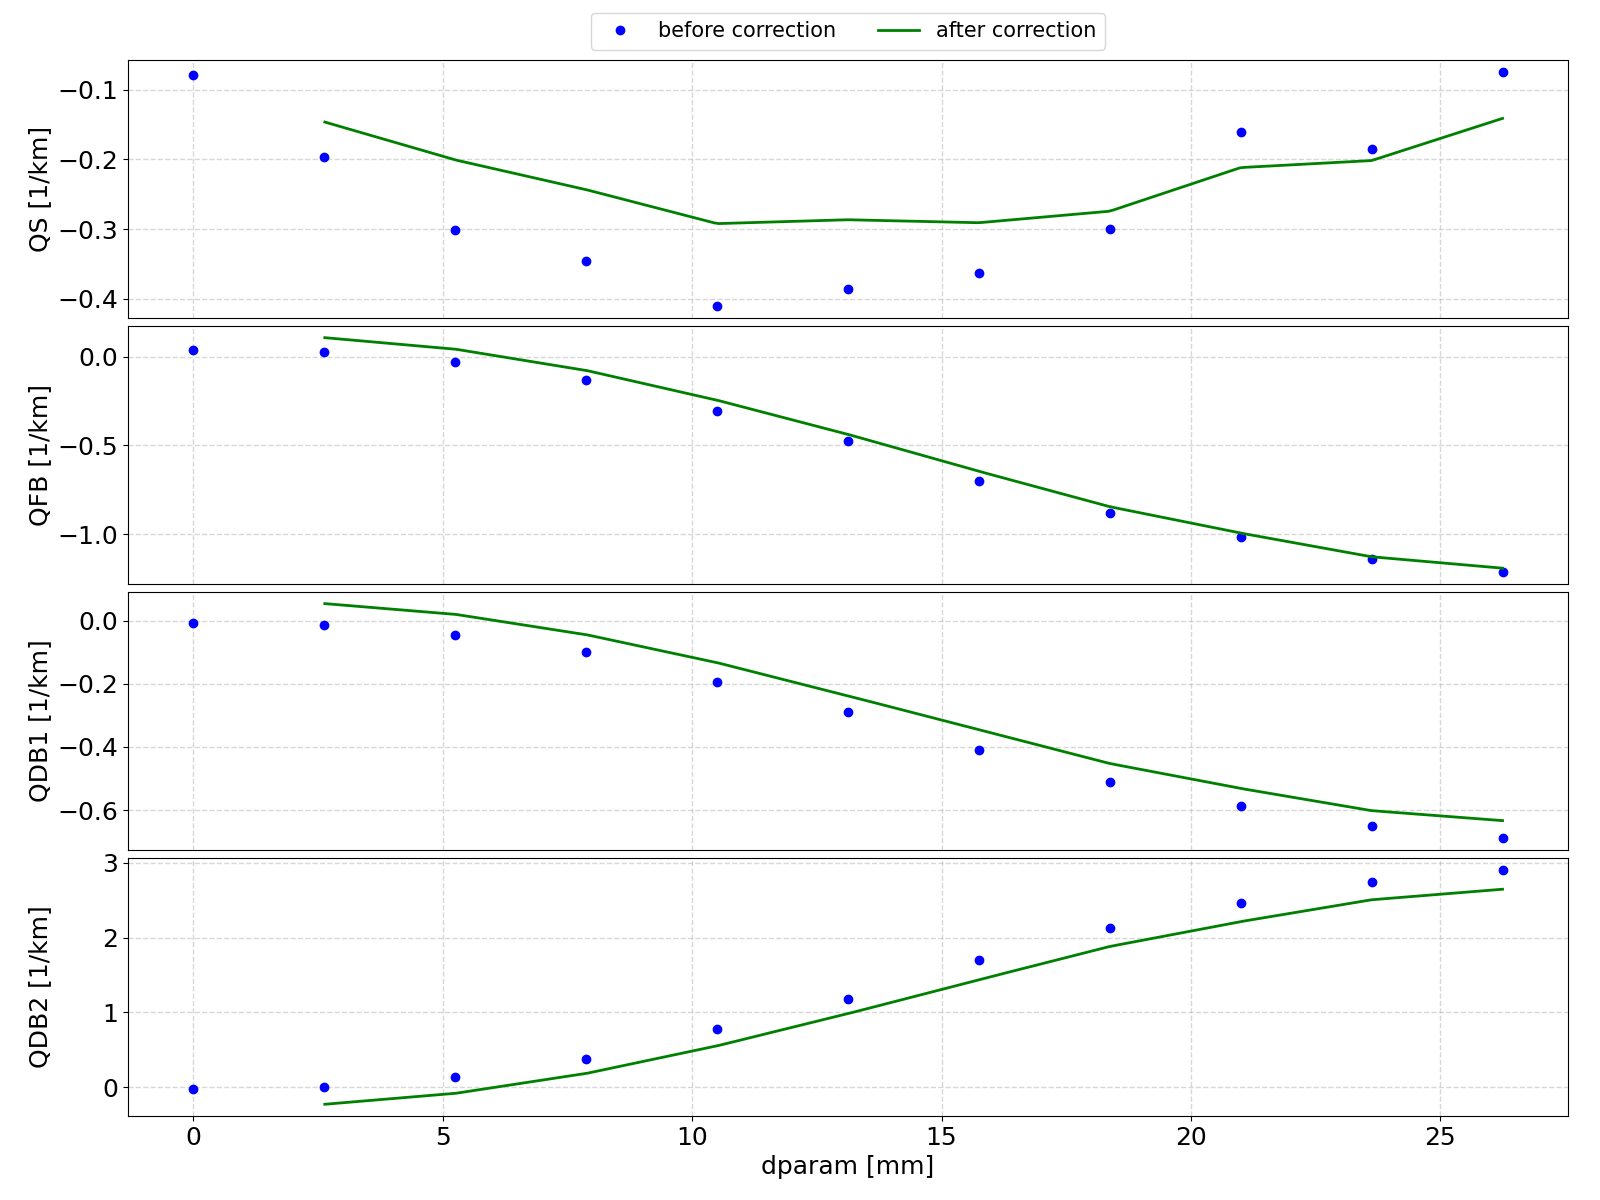
\includegraphics[width=0.8\textwidth]{2024-01-26/figures/quads_stren_with_corr.png}
            % \caption{\small{No correction}}
            \label{fig:bba}
    \end{figure} 
\end{frame}


\begin{frame}{DELTA52 - Caracterização e Correção - 23/01}
    \begin{itemize}
            \item fitting local mas com algoritmo LOCO.
    		\item Desvios de sintonia após correção (medidas):
    \end{itemize}
    \begin{figure}[H]
        	\centering
            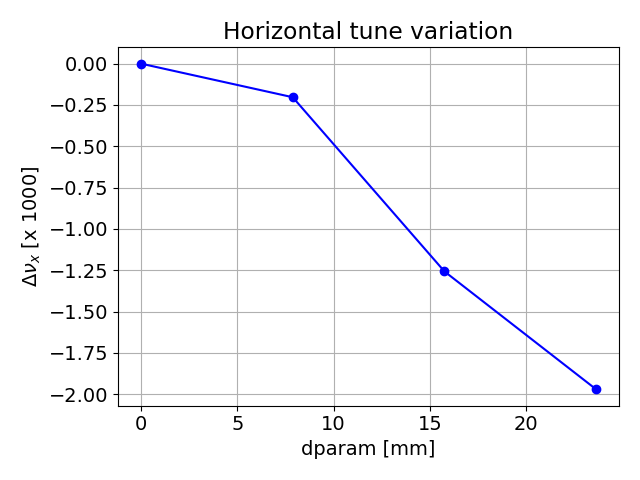
\includegraphics[height=3.5cm, width=6cm]{2024-01-26/figures/Tunex_after_loco_2401.png}\\ 
            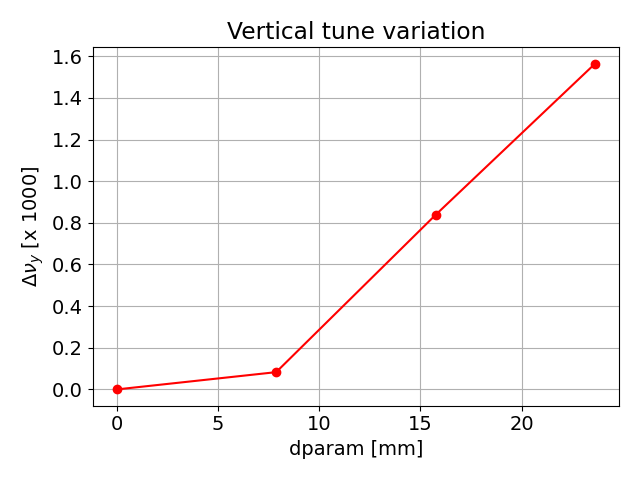
\includegraphics[height=3.5cm, width=6cm]{2024-01-26/figures/Tuney_after_loco_2401.png}\\ 
    \end{figure} 
\end{frame}


\begin{frame}{DELTA52 - Caracterização e Correção - 23/01}
    \begin{itemize}
    		\item Efeito da variação das matrizes resposta em função da corrente comprometeu o fitting. (10 mA vs 100 mA)
    \end{itemize}
    \begin{figure}[H]
        	\centering
            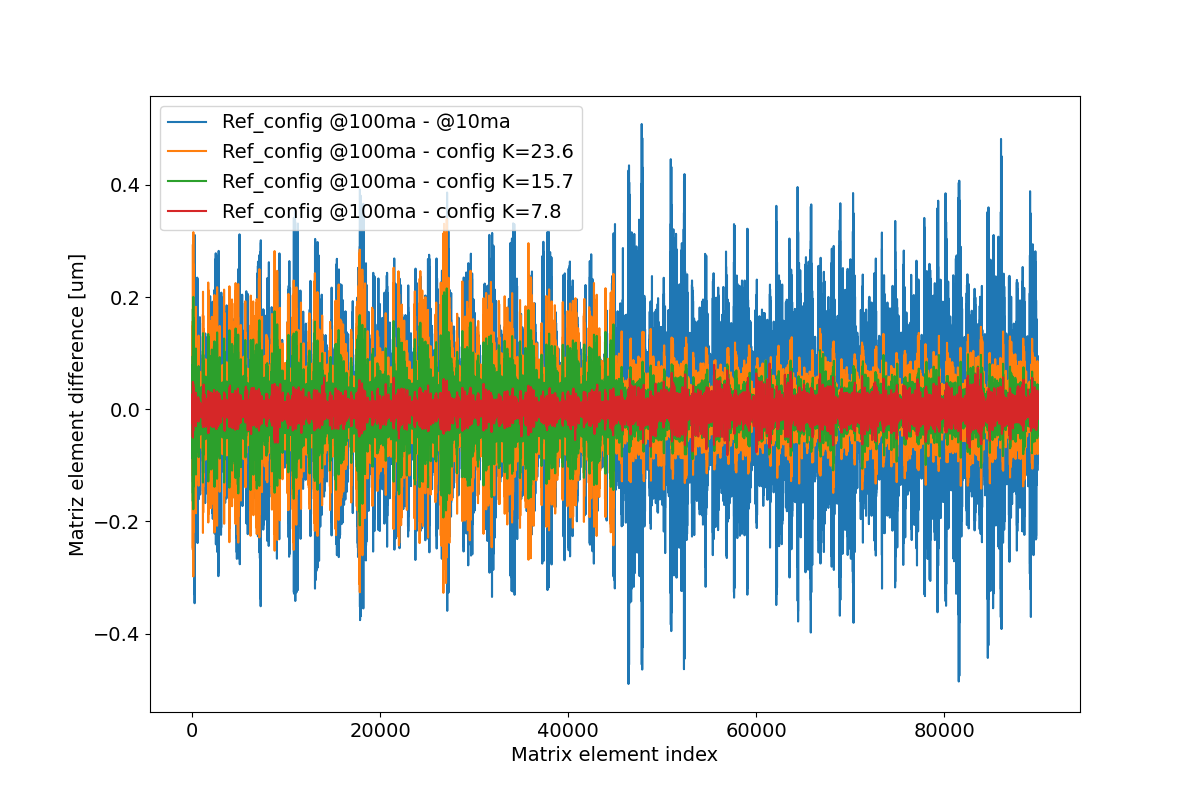
\includegraphics[height=7cm, width=9cm]{2024-01-26/figures/Matriz variation.png}\\ 
    \end{figure} 
\end{frame}


\section{Conferências e Workshops}

\begin{frame}{Conferências e Workshops}
    \begin{itemize}
            \item Low Emittance Rings 2024: "Perturbation sources and improvements of Sirius Beam Stability" (13/02-16/02 Genebra)
            \item Bunch-by-Bunch Feedback Systems and Related Beam Dynamics (03/03-06/03 Karlsruhe)
            \item Injectors for Storage Ring Based Light Sources: Apresentação entitulada: "Experience with the SIRIUS booster" (06/03-08/03 Karlsruhe)
            \item HarmonLIP 2024: Apresentação -- Predictions of slow longitudinal mode-1 instability in storage rings with harmonic cavities (Remote) (19/03-20/03 Grenoble ESRF)
    \end{itemize}
\end{frame}





\section{References}


\end{document}
